\documentclass[10pt, notumble, letterpaper]{leaflet}

\usepackage[utf8]{inputenc}
\usepackage[spanish,es-noshorthands]{babel}
\usepackage{url}
\usepackage[dvipsnames,usenames, x11names, table]{xcolor}
\usepackage{multirow}
\usepackage{array}


\definecolor{LIGHTGRAY}{gray}{.95}

\pagestyle{empty}

\title{\vspace*{3cm}\textcolor{orange}{\emph{\textbf{El 22 de noviembre vota 144 a la Asamblea ADE}}}}

\author{\textcolor{red}{\textbf{\textit{\Large{Germán Avendaño Ramírez}}}}\\\textcolor{red}{\Large{\textit{\textbf{Adriana Benavides García}}}}\\\textcolor{red}{\textit{\Large{\textbf{Helmer Avendaño Ramírez}}}}}
\date{}

\CutLine*{1}% Dotted line without scissors
\CutLine*{3}% Dotted line without scissors
\CutLine*{4}% Dotted line without scissors
\CutLine*{6}%  Dotted line with scissors

%\AddToBackground{1}{%  Background of a small page
  %\put(0,0){\textcolor{Cerulean}{\rule{\paperwidth}{\paperheight}}}}

\AddToBackground{1}{%  Background of a small page
  \put(10,500){
\includegraphics[scale=.5]{logo.png}  }}

%\AddToBackground{6}{%  Background of a small page
 % \put(0,0){\textcolor{Cyan!20}{\rule{\paperwidth}{\paperheight}}}} %YellowOrange

\AddToBackground{5}{%  Background of a small page
 \put(20,120){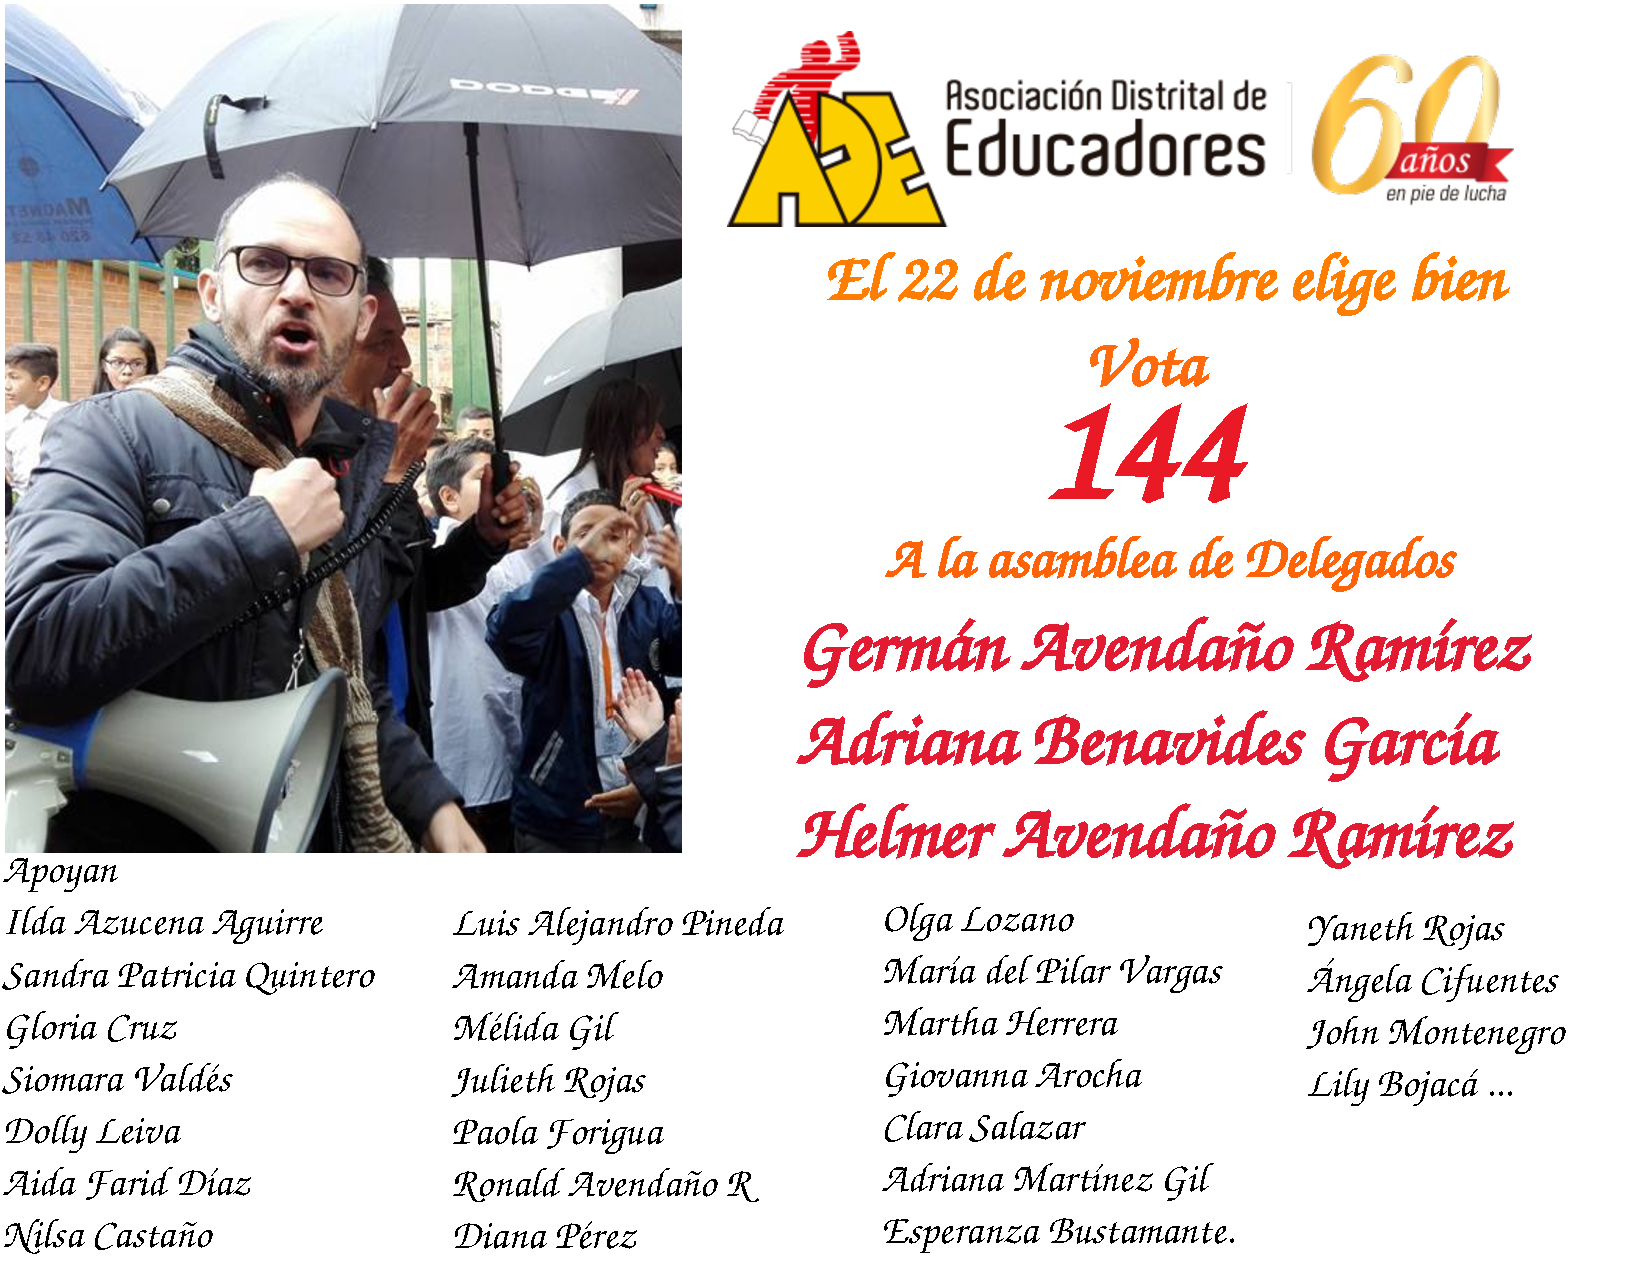
\includegraphics[scale=.675]{LogoCampana} }}

\AddToBackground{4}{%  Background of a small page
 \put(20,50){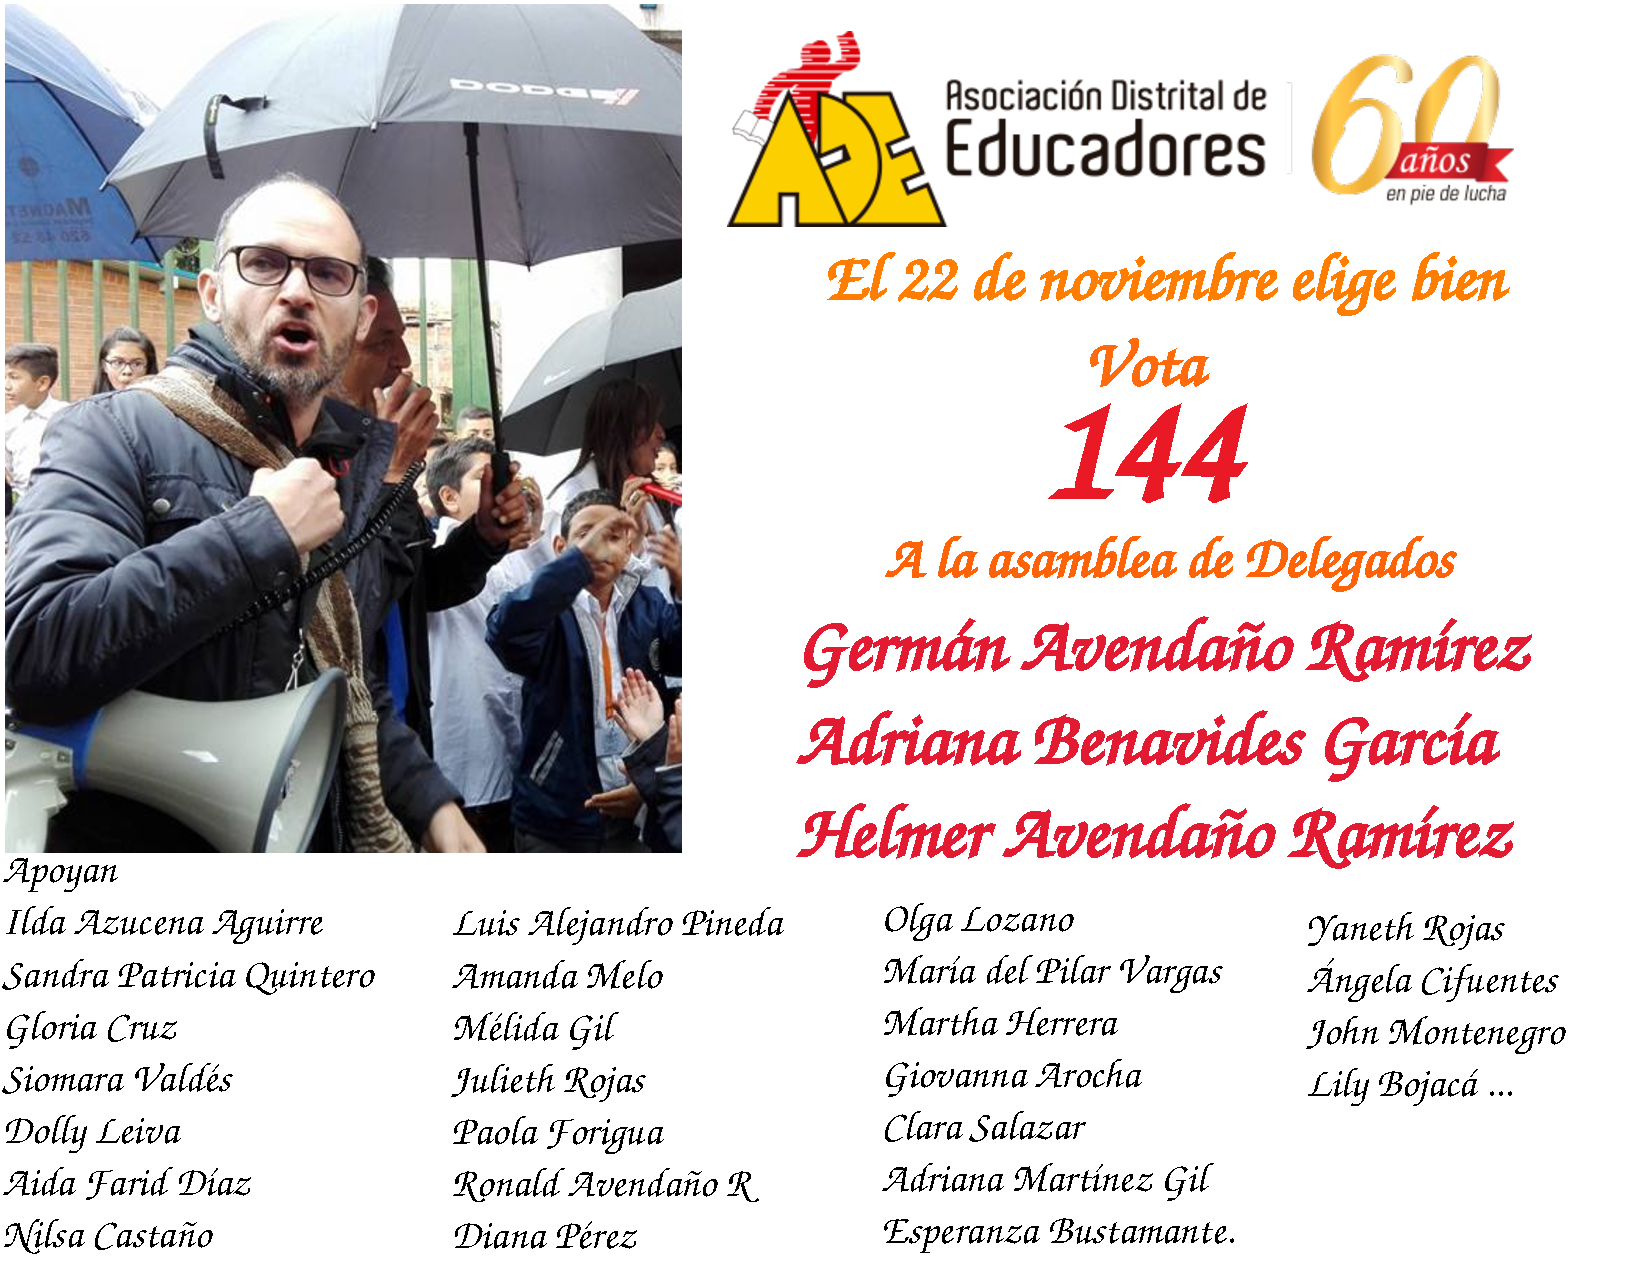
\includegraphics[scale=.55,clip=true,trim=12cm 7cm 1cm 1cm]{LogoCampana} }}

\begin{document}

\maketitle

\thispagestyle{empty}
\section*{\textcolor{red}{Propuesta de trabajo}}
Somos un grupo de maestros/as que creemos firmemente en el poder nuestro, fruto de la unidad y la organización, para librar las más duras batallas que se avecinan y confrontar así la arremetida del capital internacional y del sistema político imperante, en contra de la educación pública estatal.

Con esta idea de fondo, nos constituiremos en una alternativa de dirección para las futuras elecciones ADE. Por ahora, aspiramos a ganar un espacio en la asamblea de delegados y desde allí continuar trabajando en beneficio de nuestra organización y del magisterio en general.

Cosideramos de vital importancia que la dirección sindical sepa orientar al conjunto del magisterio de una manera clara y con argumentos que confronten las propuestas del gobierno. Por ejemplo sabemos que Colombia invierte un promedio de 1.094 dólares por año en un estudiante, mientras que los países de la OCDE invierten en promedio cerca de 8.296 dólares (7.6 veces más que Colombia) por estudiante al año según datos del año 2011. Ante el discurso del gobierno, de que estamos mal en las pruebas y que los/as maestros/as somos responsables, la dirección sindical no ha sabido dar una respuesta contundente que deje en evidencia la falacia gubernamental de que vamos a ser "el país más educado" cuando con las cifras de inversión en educación se pronostica todo lo contrario. No podemos continuar contraponiendo al discurso del gobierno una postura de desobediencia civil carente de argumentación y menos aún, podemos asumir la responsabilidad que le cabe al gobierno nacional. En este sentido creemos que podemos aportar con propuestas claras, argumentadas que nos encaminen a luchar por una mejor educación para las actuales y futuras generaciones.

Como delegados a la Asamblea ADE buscaremos:
\begin{itemize}
\item Exigirle a la administración distrital mejores condiciones para el ejercicio de nuestra labor.
\item Que se garantice el derecho a la huelga y a la protesta pacífica.
\item Velar por la no implementación de la jornada única neoliberal porque no existen las condiciones para asumirla.
\item Profundizar la democracia sindical al interior de nuestra organización
\item Articular el trabajo sindical de nuestra organización con otras organizaciones afines y movimientos sociales y populares. Unidos derrotaremos las política neoliberal que se nos quiere imponer.
\item Trabajar con y por los/as docentes que a diario defendemos la educación pública estatal desde nuestras aulas.
\item Una mejor interacción de la Asamblea con los/as afiliados/as a nuestra organización.
\item Incentivar la participación de los/as afiliados/as en la construcción de los pliegos de peticiones distritales.
\end{itemize}
\vspace{.25cm}
\fbox{
\begin{minipage}{.95\textwidth}
\begin{center}
\emph{\large El 22 de noviembre marca\\ \vspace*{.2cm} \textcolor{red}{\begin{Huge}144\end{Huge}}\\\vspace*{.2cm}en el tarjetón verde a la Asamblea ADE
}
\end{center}\end{minipage}}
\newpage
\fbox{
\begin{minipage}{.95\textwidth}
\begin{center}
\emph{\textcolor{red}{\begin{Huge}144\end{Huge}}\\\vspace*{.25cm}\large Una opción independiente a la ADE, sin compromisos burocráticos. Nuestro principal compromiso es con la defensa de la educacion pública estatal
}
\end{center}\end{minipage}}
\section{\textcolor{red}{Nuestra trayectoria}}
Los integrantes de esta lista somos hijos/as de la educación pública (literalmente), pues somos hijos/as de maestros/as y nos hemos formado en los colegios y universidades públicas. 
\subsection{\textcolor{Maroon}{Germán Avendaño Ramírez}}
Docente adscrito a la SED Bogotá desde el año 2005, nombrado mediante concurso de méritos en el colegio Arborizadora Baja I.E.D. donde he sido líder sindical por varios años y representante al comité local sindical local de Ciudad Bolívar. 
Mi historia académica es la siguiente.
\begin{itemize}
\item Lic. en matemáticas de la Universidad Distrital Francisco José de Caldas
\item M.Sc. Universidad Nacional de Colombia
\end{itemize}
Actualmente Delegado a la Asamblea ADE, donde hice parte de la Comisión de Reforma Estatutaria. Con un trabajo de más de 3 años, logramos sacar avante una reforma donde destacan los siguientes logros:
\begin{itemize}
\item Se logra poner límite al número de períodos a máximo dos consecutivos en que una persona puede ser de la Junta Directiva de la ADE.
\item Se amplía el número de delegados a la Asamblea ADE a 130 y a la junta directiva a 13, esto con el fin de garantizar una mayor participación y una mayor atención a los/as afiliados/as teniendo en cuenta el gran número de docentes que somos en Bogotá, cerca de 34.000, distribuídos en 20 localidades. 
\end{itemize}
Estos y otros logros importantes quedaron plasmados en los nuevos estatutos.

\newpage
\subsection{\textcolor{Maroon}{Adriana Benavides García}}
Nombrada desde el año 2005 en la SED Bogotá como docente de química, y, mediante concurso de méritos ahora se desempeña como coordinadora del colegio Diego Montaña Cuéllar en la localidad 5. Su formación académica es la siguiente.
\begin{itemize}
\item Licencia en Química Universidad Distrital Francisco José de Caldas
\item Especilista en análisis químico instrumental Pontificia Universidad Javeriana
\item M. Sc. Universidad Nacional de Colombia
\end{itemize}
\subsection{\textcolor{Maroon}{Helmer Avendaño Ramírez}}
Docente nombrado en Cundinamarca en el año 2007, luego mediante concurso de méritos ingresa a la SED Bogotá como coordinador en el colegio Ramón de Zubiría de la localidad de Suba.

Su formación académica es la siguiente:
\begin{itemize}
\item Licenciado en física de la Universidad Distrital Francisco José de Caldas.
\item M.Sc. Universidad Nacional de Colombia
\end{itemize}

\newpage




\newpage



\newpage



%\begin{center}
%
\includegraphics[scale=1]{LogoTEC}
%\end{center}

\end{document}